\documentclass[11pt, a4paper, titlepage, block]{article}
\usepackage{listings}
\hyphenpenalty=10000

\usepackage{graphicx}
\begin{document}
\begin{titlepage}

\newcommand{\HRule}{\rule{\linewidth}{0.5mm}} % Defines a new command for the horizontal lines, change thickness here

\center % Center everything on the page
 
%----------------------------------------------------------------------------------------
%	HEADING SECTIONS
%----------------------------------------------------------------------------------------


%----------------------------------------------------------------------------------------
%	TITLE SECTION
%----------------------------------------------------------------------------------------


%\HRule \\[0.4cm]
{ \huge \bfseries Project Report}\\[1.2cm]
%\HRule \\[0.4cm]

{\LARGE Algoritmi e Strutture Dati}\\[0.5cm]
{\large 2013/2014 summer session}
\\[1.5cm]

{\large Julian Sparber}\\[0.2cm]
{\large matr. no.: 260324}\\[1cm]
%----------------------------------------------------------------------------------------
%	AUTHOR SECTION
%----------------------------------------------------------------------------------------


%----------------------------------------------------------------------------------------
%	DATE SECTION
%----------------------------------------------------------------------------------------

%{\large \today}\\[10cm] % Date, change the \today to a set date if you want to be precise

%----------------------------------------------------------------------------------------
%	LOGO SECTION
%----------------------------------------------------------------------------------------

%\includegraphics{Logo}\\[1cm] % Include a department/university logo - this will require the graphicx package
 
%----------------------------------------------------------------------------------------

\newpage

\end{titlepage}

\section{Specifica del problema}
	Si supponga di elaborare i dati relativi ad un grafo. Le informazioni associate al problema siano: un insieme di vertici (con nomi specifcati da stringhe prive di spazi) e un insieme di archi caratterizzati da una tripla di distanze d1, d2, d3 (una tripla di numeri reali).
	\subsection{}
	Acquisisce da file le informazioni relative al grafo. Il formato del file \`{e} del tipo:\\
	\begin{tabular}{|c|c|c|c|c|}
\hline
	{\textless}No. totale dei vertici{\textgreater} & & & & \\
\hline
	{\textless}No. di vertici collegati al vertice A{\textgreater} & & & & \\
\hline
	{\textless}vertice\_A{\textgreater} & {\textless}vertice\_B{\textgreater} & {\textless}d1{\textgreater} & {\textless}d2{\textgreater} & {\textless}d3{\textgreater}\\
\hline
	{\textless}vertice\_A{\textgreater} & {\textless}vertice\_M{\textgreater} & {\textless}d1{\textgreater} & {\textless}d2{\textgreater} & {\textless}d3{\textgreater}\\
\hline
	... & & & &\\
\hline
	{\textless}vertice\_A{\textgreater} & {\textless}vertice\_Z{\textgreater} & {\textless}d1{\textgreater} & {\textless}d2{\textgreater} & {\textless}d3{\textgreater}\\
\hline
	{\textless}No. di vertici collegati al vertice B{\textgreater} & & & &\\
\hline
	{\textless}vertice\_B{\textgreater} & {\textless}vertice\_C{\textgreater} & {\textless}d1{\textgreater} & {\textless}d2{\textgreater} & {\textless}d3{\textgreater}\\
\hline
	{\textless}vertice\_B{\textgreater} & {\textless}vertice\_X{\textgreater} & {\textless}d1{\textgreater} & {\textless}d2{\textgreater} & {\textless}d3{\textgreater}\\
\hline
	... & & & &\\
\hline
\end{tabular}
	\subsection{}
	Inserisce i dati acquisiti in una opportuna struttura dati.
	\subsection{}
	Dati un vertice sorgente, uno destinazione e una tipologia di distanze (d1 oppure d2 oppure d3) inseriti dall'utente, calcola il percorso pi\`{u} breve tra sorgente e destinazione, mostrando a
monitor tale percorso e la relativa distanza.
	\subsection{}
	Dato un vertice specificato dall'utente, calcola la media e la mediana della distanze minime che separano tale vertice da tutti gli altri vertici del grafo, in base alle tipologie di distanza d1, d2 e d3.\\ \\
	Per quanto riguarda l'analisi teorica si devono studiare le complessit\`{a} degli algoritmi di acquisizione del file (punto 2), calcolo del percorso pi\`{u} breve tra due vertici (punto 3) e calcolo di media e mediana (punto 4).\\
	Per quanto riguarda il punto 4 si deve anche verificare sperimentalmente la complessit\`{a} delcalcolo di media e mediana, generando casualmente una sequenza di distanze (di N numeri reali) da fornire come input all'algoritmo per valori crescenti di N.

	\newpage
\section{Progettazione dell problema}
Ogni carattere letto dal file viene validato immediatamente. Il nodo e l'arco preso da ognuna delle righe viene salvato in una struttura dinamica di questo tipo: \\\\
\{\\
\indent nome del nodo,\\
\indent archi del nodo,\\
\indent minima distanza,\\
\indent parente del nodo,\\
\indent nodo successivo; \\
\}\\\\
e gli archi vengono salvati in una struttura di questo tipo:\\\\
\{\\
\indent nome del nodo di destinazione,\\
\indent nodo di destinazione,\\
\indent la tripla della distanza,\\
\indent arco successivo;\\
\}\\\\
Un vertice sorgente, un vertice destinazione e una tipologia di distanze (d1 oppure d2 oppure d3) viene chiesto all'utente.\\
Visto che i valori in questo grafo sono distanze, non possono essere negativi. Per questa ragione l'algoritmo di Dijkstra \`{e} una buona scelta.\\\\

La mediana viene calcolata con quickselect, un'algoritmo randomizzato che trova il k-esimo elemento di una struttura disordinata con n elementi eseguendo in O(n$^2$) nel caso pessimo e O(n) nel caso ottimo.\\\\ 

Quickselect \`{e} relativamente semplice da implementare, e, se implementato correttamente, leggermente pi\`{u} veloce di heapselect.\\
All'utente viene mostrato il percorso pi\`{u} breve tra i nodi sorgente e destinazione definiti dall'utente e anche la media e la mediana delle distanze minime dal nodo sorgente a tutti gli altri vertici del grafo.
	\newpage
\section{Valutazione della complessit\`{a} del programma}
Visto che l' algoritmo viene applicato su struttura a grafo, la complessit\`{a} pu\`{o} essere espressa in 
funzione del numero di vertici e di archi del grafo stesso. A questo scopo verr\`{a} indicato con $|$V$|$ il 
numero di vertici e con $|$E$|$ (edges) il numero di tutti gli archi.\\
\\
La complessit\`{a} dell'algoritmo di acquisizione:\\
\indent T($|$V$|$, $|$E$|$) = 1+ $|$V$|$ + $|$E$|$ = O($|$V$|$ + $|$E$|$)\\
La complessit\`{a} dell'algoritmo per calcolare il percorso pi\`{u} breve tra due vertici (Algoritmo di Dijkstra):\\
\indent T ($|$V$|$, $|$E$|$) = O($|$V$|$ x log $|$V$|$ + $|$E$|$)\\
La complessit\`{a}  dell'algoritmo per calcolare la media:\\
\indent T($|$V$|$, $|$E$|$) = O($|$V$|$)\\
La complessit\`{a} dell'algoritmo per calcolare la mediana (quickselect):\\
\indent Caso ottimo:\\
\indent \indent T($|$V$|$, $|$E$|$) = $|$V$|$ + $|$V$|$ + T($|$V$|$ / 2) = O($|$V$|$)\\
\indent Caso pessimo:\\
\indent \indent T($|$V$|$, $|$E$|$) = $|$V$|$ + $|$V$|$ + T($|$V$|$ - 1) = O($|$V$|$2)\\
	\newpage
\section{Valutazione sperimentale della complessit\`{a} del calcolo di media e mediana}
Nei risultati della valutazione sperimentale si vede che la complessit\`{a} del calcolo della media \`{e} O($|$V$|$).
\begin{figure}[htp]
\centering
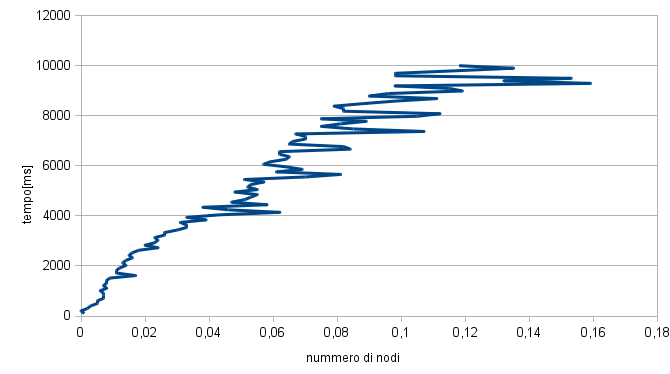
\includegraphics[scale=0.80]{img/calcolo_media.png}
\caption{complessit\`{a} del calcolo di media}
\end{figure}
\newpage
Anche il risultato dalla valutazione sperimentale del calcolo della mediana non sorprende. Qui si vede il confronto dei calcoli di media e di mediana. 
La complessit\`{a} varia molto perch\`{e} quickselect \`{e} casuale quindi dipende molto dal vertice di partenza.
\begin{figure}[htp]
\centering
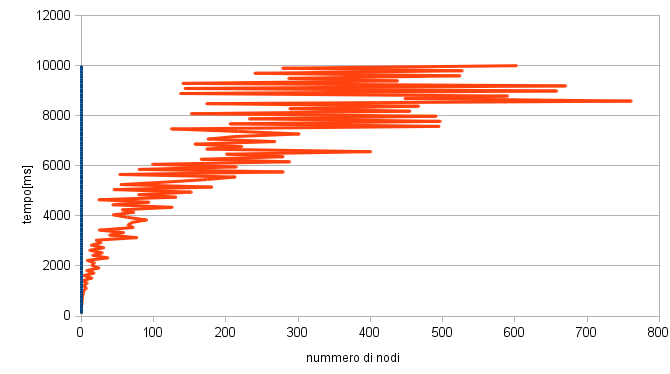
\includegraphics[scale=0.80]{img/calcolo_mediana.png}
\caption{complessit\`{a} del calcolo di media(blue) e mediana(rosso)}
\end{figure}

\end{document}